%!TEX TS-program = xelatex
\documentclass[]{friggeri-cv}
\usepackage{afterpage}
\usepackage{hyperref}
\usepackage{color}
\usepackage{xcolor}
\usepackage{smartdiagram}
\usepackage{fontspec}
% if you want to add fontawesome package
% you need to compile the tex file with LuaLaTeX
% References:
%   http://texdoc.net/texmf-dist/doc/latex/fontawesome/fontawesome.pdf
%   https://www.ctan.org/tex-archive/fonts/fontawesome?lang=en
%\usepackage{fontawesome}
%\usepackage[backend=biber]{biblatex}
%\usepackage[backend=biber,style=unsrt]{biblatex}

\usepackage{metalogo}
\usepackage{dtklogos}
\usepackage[utf8]{inputenc}
\usepackage{tikz}
\usetikzlibrary{mindmap,shadows}
\hypersetup{
    pdftitle={},
    pdfauthor={},
    pdfsubject={},
    pdfkeywords={},
    colorlinks=false,           % no lik border color
    allbordercolors=white       % white border color for all
}
\smartdiagramset{
    bubble center node font = \footnotesize,
    bubble node font = \footnotesize,
    % specifies the minimum size of the bubble center node
    bubble center node size = 0.5cm,
    %  specifies the minimum size of the bubbles
    bubble node size = 0.5cm,
    % specifies which is the distance among the bubble center node and the other bubbles
    distance center/other bubbles = 0.3cm,
    % sets the distance from the text to the border of the bubble center node
    distance text center bubble = 0.5cm,
    % set center bubble color
    bubble center node color = pblue,
    % define the list of colors usable in the diagram
    set color list = {lightgray, materialcyan, orange, green, materialorange, materialteal, materialamber, materialindigo, materialgreen, materiallime},
    % sets the opacity at which the bubbles are shown
    bubble fill opacity = 0.6,
    % sets the opacity at which the bubble text is shown
    bubble text opacity = 0.5,
}

\addbibresource{bibliography.bib}
\RequirePackage{xcolor}
\definecolor{pblue}{HTML}{0395DE}

\begin{document}
\header{Virgile}{Daugé}
      {Ingénieur en Informatique}
      
% Fake text to add separator      
\fcolorbox{white}{gray}{\parbox{\dimexpr\textwidth-2\fboxsep-2\fboxrule}{%
.....
}}
\smartdiagramset{distance center/other bubbles=0.5cm,bubble center node size=1cm,bubble node size=1.4cm}
% In the aside, each new line forces a line break
\begin{aside}
  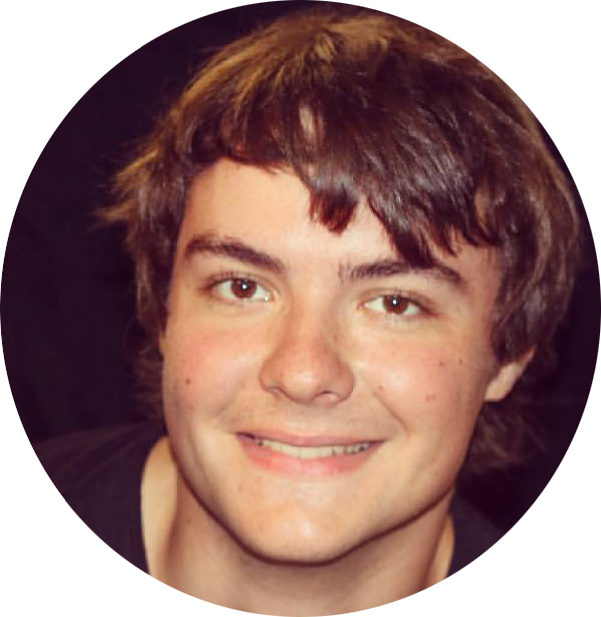
\includegraphics[scale=0.2]{img/photoCV.png}
  \section{Adresse}
    27 rue Christian Pfister
    Nancy
    54000
    ~
  \section{Tel \& Skype}
    +33 63 46 19 65
    virgile.dauge.tn
    ~
  \section{Mail}
    \href{mailto:virgile.dauge@telecomnancy.net}{\textbf{virgile.dauge@}\\telecomnancy.net}
    ~
  \section{Web \& Git}
    \href{http://www.virgiledauge.fr}{virgiledauge.fr}
    \href{https://github.com/virgileTN}{github.com/virgileTN}
    ~
  % use  \hspace{} or \vspace{} to change bubble size, if needed
  \section{Programmation}
    \smartdiagram[bubble diagram]{
        \textbf{Algo},
        \textbf{\hspace{6mm}C/C++\hspace{6mm}}\\\textbf{},
        \textbf{ROS},
        \textbf{Python},
        \textbf{}\\\textbf{\LaTeX}
    }
    ~
\end{aside}
~
\section{Expérience Professionnelle}
\begin{entrylist}
  \entry
    {04/17 - 2020}
    {Thèse}
    {Loria - Université de Lorraine}
    {Systèmes Cyber-Physiques autonomes et communicants en milieux hostiles. Application à l’exploration par robots mobiles. \\
    Conception d'algorithmes adaptatifs, produisant des résultats de qualité/précision variables selon les besoins et limitations du système. L'application visée, centrale dans le domaine des systèmes cyber-physiques mobiles (drones, robots,...), est la reconstruction tridimensionnelle de l’environnement dans lequel les agents évoluent. Elle concerne des zones en extérieur comme en intérieur, non maîtrisées (pas de connaissances extérieures de positionnement, de carte etc...). La reconstruction peut être un objectif en soi, mais peut également être une tâche interne utile à la navigation des agents mobiles et à leur prise de décision. La qualité de reconstruction se doit d'être modulable (précision, densité) afin de limiter la quantité de calculs et ainsi respecter les contraintes temps-réel imposées pour une plateforme autonome. La coopération de différents éléments et de leurs composants(capteurs, actionneurs, calculateurs, interfaces de communication) est étudiée dans l'objectif d'augmenter la robustesse du système tout en augmentant la précision des résultats. 
  }
  \entry
    {04/16 - 09/16}
    {Stage ingénieur}
    {Institut national de recherche en informatique et en automatique}
    {Conception et développement d'un contrôleur d'hexapode (c++) basé sur les retours de forces fournis pas des capteurs situés aux extrémités des pattes. La réalisation du contrôleur à nécessité la conception et l'implémentation d'une solution de cinématique inverse, permettant le contrôle précis de la trajectoire de chaque patte. Le nouveau contrôleur permet à l'hexapode de traverser sans encombres un terrain composé d'obstacles multiples, effectuant des trajectoires jusqu'à 39\% plus lisses.\href{https://www.youtube.com/watch?v=-7WJkv4gbe4}{vidéo}\cite{hexapod}.}
  \entry
    {07/15 - 08/15}
    {Stage en mobilité internationale}
    {Parallel Geometry, Montréal, Canada}
    {Le stage a consisté en l'analyse puis l'audit du nouveau format de fichiers pour l'impression 3D, le format AMF(Additive Manufacturing File Format) ainsi que de la librairie (c++) l'accompagnant. L'analyse portait plus particulièrement sur le stockage de volumes dit "solides" comportant à la fois les données de surface et la structure interne d'un objet. Les principales techniques de représentation du solide ont été passées en revue, après avoir mis en place un environnement de test pour chacune d'elles. Le rapport réalisé a servi par la suite à la révision de la norme dans le cadre du workitem ASTM WK48549\cite{AMF}.}
  \entry
    {07/13 - 08/13}
    {Stage DUT}
    {Centre National de la Recherche Scientifique, Nancy, France}
    {Conception et réalisation de l'interface électronique et du programme de contrôle d'une ligne d'extraction/purification des gaz de roche.}
  \entry
    {01/13 - 07/13}
    {Chef de projet concours de robotique national}
    {IUT Nancy-Brabois, France}
    {Construction et management d'une équipe de 12 étudiants, qui a réalisé un robot Linux Embarqué(c/c++) comprenant un FPGA (VHDL) pour le traitement des signaux. Le robot a remporté tous les matchs jusqu'à la perte d'un composant électronique critique.}
\end{entrylist}
\newpage
\section{Expérience Associative}
\begin{entrylist}
  \entry
  {2014 - 2015}
  {Responsable communication}
  {Cercle des élèves de Télécom Nancy}
  {Principal interlocuteur entre le bureau des étudiants et les partenaires extérieurs. Cet engagement à  nécessité la négociation de contrats ainsi que de nombreuses interventions devant un public large.\\}
  \entry
  {2014 - 2015}
  {Club Intégration \& Jeux}
  {Cercle des élèves de Télécom Nancy}
  {Organisation d'événements regroupant plus de 150 étudiants.\\}
  \entry
  {2014 - 2018}
  {Club Photo/Vidéo}
  {Cercle des élèves de Télécom Nancy}
  {La réalisation de nombreux montages photo et vidéos complètent ma passion pour la photo, et m'ont appris à concevoir et réaliser de manière efficace des supports de communication.\\}
\end{entrylist}

\section{Formation}
\vspace{0.3cm}
\begin{entrylist}
  \entry
    {2013 - 2016}
    {Ecole d'ingénieur en informatique}
    {Télécom Nancy, Nancy, France}
    {La formation proposée à Télécom Nancy est généraliste, nous donnant les outils nécessaires à une bonne compréhension des technologies, mais surtout une forte capacité d'adaptation. Effectuer la spécialisation logiciels embarqués m'a permis de compléter les connaissances abordées en DUT tout en en découvrant d'autres, comme l'intelligence artificielle, pour laquelle je développe un intérêt croissant.\\}
  \entry
    {2011 - 2013}
    {DUT Génie électrique et informatique industrielle}
    {IUT Nancy-Brabois, France}
    {Allant de l'électrotechnique à la programmation orientée objet, en passant par l'électronique, les compétences acquises en DUT GEII sont un plus pour la robotique.\\}
  \entry
    {2011}
    {Baccalauréat Scientifique}
    {Lycée E.S.T.I.C., Saint-Dizier, France}
    {Formation scientifique option sciences de l'ingénieur. les bases de la mécanique, de l'électricité et de programmation abordées m'ont donné le goût de l'ingénierie. Mention Bien.\\}
\end{entrylist}
\smartdiagramset{distance center/other bubbles=0.5cm,bubble center node size=1cm,bubble node size=1.4cm}
\begin{aside}
~
~
~
  \section{Compétences personnelles}
    \smartdiagram[bubble diagram]{
        \textbf{Curiosité},
        \textbf{\vspace{1mm}Initiative\vspace{1mm}},
        \textbf{Résolution}\\\textbf{de}\\\textbf{problèmes},
        \textbf{Organisation},
        \textbf{}\\\textbf{\vspace{1mm}Créativité\vspace{5mm}},
        \textbf{Jovial}
    }
    ~
  \section{OS préférés}
    \textbf{GNU/Linux}
\includegraphics[scale=0.40]{img/5stars.png}
    \textbf{Windows}
\includegraphics[scale=0.40]{img/2stars.png}
    \textbf{MacOS}
\includegraphics[scale=0.40]{img/1stars.png}
    ~
  \section{Langues}
    \textbf{French}
\includegraphics[scale=0.40]{img/5stars.png}
    \textbf{English}
\includegraphics[scale=0.40]{img/4stars.png}
    ~
\end{aside}


\section{Certifications}
\begin{entrylist}
  \entry
    {01/2013}
    {TOEIC}
    {850/990}
    {}
\end{entrylist}
\newpage
\section{Centres d’intérêt}
\begin{entrylist}
  \entry
    {}
    {Robotique}
    {}
    {\emph{J'ai développé au fur et a mesure de mes études un intérêt particulier pour la robotique. J'ai eu notamment l'occasion d'effectuer différentes réalisations dans le cadre de concours ou de projets personnels.\\}}
    \entry
    {}
    {Intelligence artificielle}
    {}
    {\emph{Mon intérêt pour l'intelligence artificielle m'a amené à réaliser différents projets, et à poursuivre la lecture d'ouvrages spécialisés \cite{IAProg}\cite{IABase}.\\}}
    
    \entry
    {}
    {Musique}
    {}
    {\emph{Pratiquant la guitare depuis des années, la musique fait partie intégrante de mes journées. Il m'arrive également de composer de la musique électronique.\\}}
    
    \entry
    {}
    {Photographie \& design}
    {}
    {\emph{Après avoir découvert la photographie via la couverture d'événements pour une association étudiante, j'ai pu concrétiser ma passion récemment par l'acquisition d'un reflex Canon760d. Je développe progressivement des compétences en montage photo et vidéo tout en réalisant divers contenus créatifs (infographies, affiches, diagrammes, logos...).\\}}
    
    
\end{entrylist}

\section{Bibliographie}
\printbibliography[heading=none]

\begin{flushleft}
\emph{\today}
\end{flushleft}
\begin{flushright}
\emph{Virgile Daugé}
\end{flushright}

\end{document}
